\chapterimage{orange2.jpg} % Chapter heading image
\chapterspaceabove{6.75cm} % Whitespace from the top of the page to the chapter title on chapter pages
\chapterspacebelow{7.25cm} % Amount of vertical whitespace from the top margin to the start of the text on chapter pages

\chapter{Input-Output Stability}\index{Input-Output Stability}

\section{Overview}\index{Overview}

So far, stability was studied using Lyapunov functions focusing on internal states. Input-Output (I/O) Stability, in contrast, studies how bounded inputs produce bounded outputs using the mapping $y = H(u)$. It treats the system as a black box without considering internal states.  

\begin{center}
\begin{tikzpicture}[auto, node distance=1.5cm, thick]
  \node (u) {$u(t)$};
  \node[draw, rectangle, minimum height=1.5cm, minimum width=2.5cm, right=of u] (H) {$H$};
  \node (y) [right=of H] {$y(t)$};
  \draw[->] (u) -- (H);
  \draw[->] (H) -- (y);
\end{tikzpicture}
\end{center}

\section{Function Spaces}\index{Function Spaces}

So far we studied vector spaces of finite-dimensional vectors.  
Now we study \textbf{function spaces}, where the elements are \emph{functions} instead of vectors.  

\begin{definition}[Function space]
A \emph{function space} is a set of functions from a domain (e.g.\ time, $\mathbb{R}_{\geq 0}$) into a codomain (e.g.\ $\mathbb{R}^q$) that is equipped with additional structure, such as operations (addition, scalar multiplication) and possibly a norm or inner product.  
For example, we may consider
\[
u:\mathbb{R}_{\geq 0} \to \mathbb{R}^q, 
\quad 
u(t) =
\begin{bmatrix}
u_1(t) \\ \vdots \\ u_q(t)
\end{bmatrix}.
\]
\end{definition}

\subsection{$L_p$ Spaces}

A particularly important class of function spaces in analysis and control are the $L_p$ spaces.

\begin{definition}[$L_p$ space]
For $1 \leq p < \infty$, the space $L_p(0,\infty;\mathbb{R}^q)$ is defined as
\[
L_p = \Big\{ u:\mathbb{R}_{\geq 0}\to \mathbb{R}^q \;\Big|\;
\int_{0}^{\infty} \|u(t)\|^p \, dt < \infty \Big\}.
\]
The corresponding norm is
\[
\|u\|_{L_p} = \left( \int_{0}^{\infty} \|u(t)\|^p \, dt \right)^{1/p}.
\]
\end{definition}

\begin{definition}[$L_2$ space]
The \emph{square-integrable space} is the case $p=2$:
\[
L_2(0,\infty;\mathbb{R}^q) 
= \Big\{ u:\mathbb{R}_{\geq 0}\to \mathbb{R}^q \;\Big|\;
\int_{0}^{\infty} \|u(t)\|^2 \, dt < \infty \Big\}.
\]
The norm
\[
\|u\|_{L_2} = \left( \int_{0}^{\infty} \|u(t)\|^2 \, dt \right)^{1/2}
\]
represents the \textbf{energy} of the signal.
\end{definition}

\begin{definition}[$L_\infty$ space]
The \emph{essentially bounded space} is defined as
\[
L_\infty(0,\infty;\mathbb{R}^q) 
= \Big\{ u:\mathbb{R}_{\geq 0}\to \mathbb{R}^q \;\Big|\;
\sup_{t \geq 0} \|u(t)\| < \infty \Big\}.
\]
The norm
\[
\|u\|_{L_\infty} = \sup_{t \geq 0} \|u(t)\|
\]
represents the \textbf{maximum amplitude} of the signal.
\end{definition}

\begin{remark}
\begin{itemize}
\item  $L_2$ is widely used to measure signal energy (that's why used in stability analysis).  
\item  $L_\infty$ is used to measure boundedness or peak values of signals.  
\item  In general, $L_p$ spaces allow us to study signals with different growth and smoothness properties, and they provide the foundation for many results in control and signal processing.
\end{itemize}
\end{remark}

\begin{proposition}[Hölder’s inequality]
Let $p,q > 1$ with $\tfrac{1}{p}+\tfrac{1}{q}=1$.  
If $f \in L_p(0,T)$ and $g \in L_q(0,T)$, then $fg \in L_1(0,T)$ and 
\[
\int_{0}^{T} |f(t)g(t)| \, dt 
\;\leq\;
\left( \int_{0}^{T} |f(t)|^p \, dt \right)^{1/p}
\left( \int_{0}^{T} |g(t)|^q \, dt \right)^{1/q}.
\]
\end{proposition}

\begin{proposition}[Minkowski’s inequality]
For $1 \leq p < \infty$, if $f,g \in L_p(0,T)$, then
\[
\|f+g\|_{L_p} \;\leq\; \|f\|_{L_p} + \|g\|_{L_p}.
\]
Thus $\|\cdot\|_{L_p}$ defines a norm on $L_p$.
\end{proposition}

\subsection{Extended Spaces}\index{Function Spaces!Extended}

\begin{definition}[Truncation operator]
Let $X$ be a function space on $[0,\infty)$.  
For $T>0$, the \emph{truncation operator} $P_T:X \to X$ is defined by
\[
(P_Tu)(t) =
\begin{cases}
u(t), & 0 \leq t \leq T,\\[6pt]
0, & t > T.
\end{cases}
\]
\end{definition}

\begin{definition}[Extended space]
Let $X$ be a function space on $[0,\infty)$.  
The \emph{extended space} $X_e$ is defined as
\[
X_e = \big\{ u:[0,\infty)\to\mathbb{R}^q \;\big|\; 
P_T u \in X \;\; \text{for all } T>0 \big\}.
\]
In words: $u \in X_e$ if \textbf{every finite-time truncation} of $u$ belongs to $X$.
\end{definition}

\begin{example}
If $X = L_2(0,\infty)$, then
\[
X_e = \{ u:[0,\infty)\to \mathbb{R}^q \mid u \in L_2(0,T) \;\;\forall T>0\}.
\]
Thus $X_e$ contains all signals that have \textbf{finite energy on every bounded interval}, even if their total energy on $[0,\infty)$ is infinite.  
For example, $u(t)=1$ is not in $L_2(0,\infty)$, but $u \in (L_2)_e$ since its truncation to any finite interval lies in $L_2(0,T)$.
\end{example}

\begin{remark}
The extended space $X_e$ enlarges $X$ by admitting signals that are locally in $X$ but not globally.  
This is useful in control theory because real signals are often studied over finite horizons.
\end{remark}

\section{Input-Output Stability}\index{Input-Output Stability}

\begin{definition}[Mapping]
The mathematical representation of a physical system is defined as a mapping
\[
H: X_e \to X_e
\]
that satisfies the \textbf{causality condition}:
\[
(Hu)_T = \big(H(u_T)\big)_T, \qquad \forall u \in X_e, \; T>0,
\]
where $X_e$ is the space consisting of all functions whose truncation belongs to $X$.
\end{definition}

\begin{example}
Consider the first-order causal system:
\[
\dot{y}(t) + y(t) = u(t), \qquad y(0) = 0.
\]

Let the input $u(t)$ be a step function. Its truncated version at $T=4$ is denoted $u_T(t)$. Then the system outputs satisfy the causality condition:
\[
(Hu)_T = (H(u_T))_T.
\]

\begin{center}
\begin{tikzpicture}[auto, node distance=1.5cm, thick]
  % First: full input
  \node (u) {$u(t)$};
  \node[draw, rectangle, minimum height=1.5cm, minimum width=2.5cm, right=of u] (H) {$H$};
  \node (y) [right=of H] {$(Hu)(t)$};
  \draw[->] (u) -- (H);
  \draw[->] (H) -- (y);
\end{tikzpicture}

\vspace{1cm}

\begin{tikzpicture}[auto, node distance=1.5cm, thick]
  % Second: truncated input
  \node (uT) {$u_T(t)$};
  \node[draw, rectangle, minimum height=1.5cm, minimum width=2.5cm, right=of uT] (H) {$H$};
  \node (yT) [right=of H] {$(H(u_T))(t)$};
  \draw[->] (uT) -- (H);
  \draw[->] (H) -- (yT);
\end{tikzpicture}
\end{center}

\begin{center}
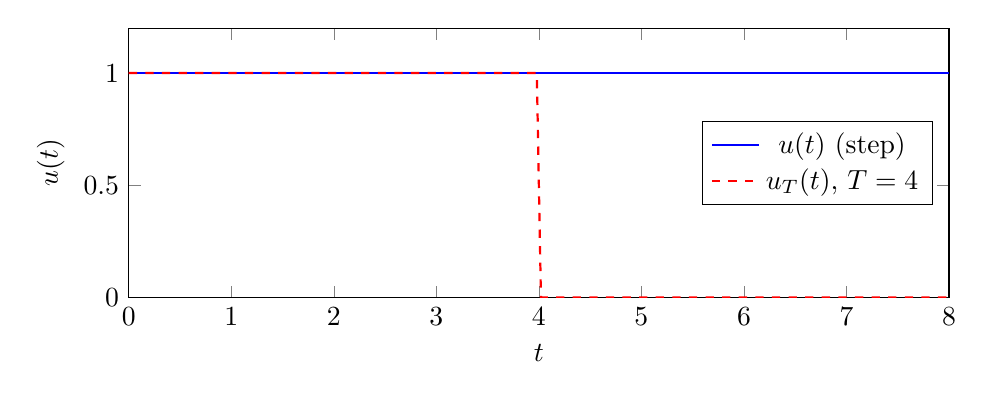
\begin{tikzpicture}
\begin{axis}[
    width=12cm, height=5cm,
    xlabel={$t$}, ylabel={$u(t)$},
    xmin=0, xmax=8, ymin=0, ymax=1.2,
    samples=200, domain=0:8,
    legend style={at={(0.98,0.5)},anchor=east}
]
\addplot[blue, thick] {x>=0 ? 1 : 0}; 
\addlegendentry{$u(t)$ (step)}

\addplot[red, dashed, thick] {x<=4 ? 1 : 0}; 
\addlegendentry{$u_T(t)$, $T=4$}
\end{axis}
\end{tikzpicture}

\vspace{0.5cm}

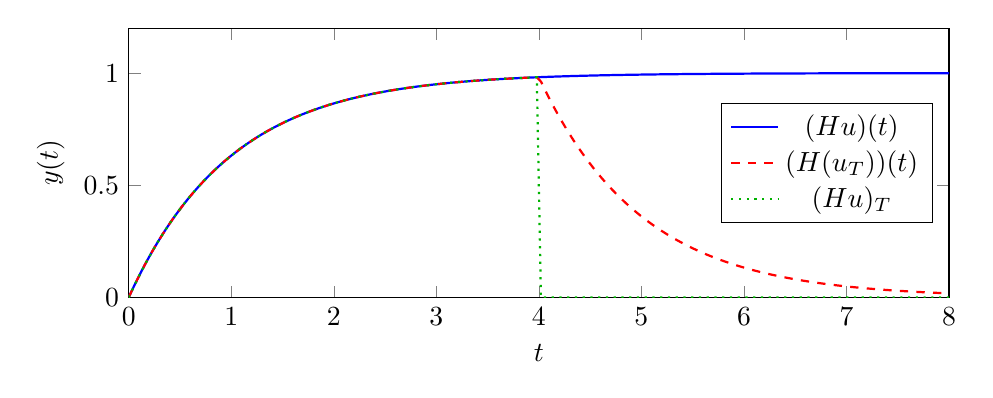
\begin{tikzpicture}
\begin{axis}[
    width=12cm, height=5cm,
    xlabel={$t$}, ylabel={$y(t)$},
    xmin=0, xmax=8, ymin=0, ymax=1.2,
    legend style={at={(0.98,0.5)},anchor=east}
]
% Full system response
\addplot[blue, thick, samples=200, domain=0:8] {1 - exp(-x)};
\addlegendentry{$(Hu)(t)$}

% Truncated input system response
\addplot[red, dashed, thick, samples=200, domain=0:8] {x<=4 ? (1 - exp(-x)) : (1 - exp(-4))*exp(-(x-4))};
\addlegendentry{$(H(u_T))(t)$}

% Output truncation
\addplot[green!70!black, dotted, thick, samples=200, domain=0:8] {x<=4 ? (1 - exp(-x)) : 0};
\addlegendentry{$(Hu)_T$}
\end{axis}
\end{tikzpicture}
\end{center}
\end{example}

\begin{remark}
For a causal system, the output at any time $t$ depends only on the input values up to that time. Therefore, if we truncate the input at time $T$ to obtain $u_T(t)$, the resulting output $(H(u_T))(t)$ matches the original output $(Hu)(t)$ for all $t \le T$. Moreover, truncating the original output at $T$, i.e., $(Hu)_T$, gives exactly the same signal. This property formally captures the essence of input-output causality.
\end{remark}

\begin{definition}[Finite-Gain System]
A system $H$ is said to have a \textbf{finite gain} if there exist constants 
\(\gamma(H) < \infty\) (called the \emph{gain} of $H$) and \(\beta \in \mathbb{R}^+\) such that, for all inputs \(u \in X_e\),
\[
\| Hu \|_X \le \gamma(H) \, \| u \|_X + \beta.
\]

Here, \(\beta\) is a bias term which may be nonzero even when \(u = 0\).  
If \((Hu) = 0\) whenever \(u = 0\), then \(\beta = 0\), and the gain can be calculated as
\[
\gamma(H) = \sup_{u \neq 0} \frac{\| (Hu)_T \|_X}{\| u_T \|_X}.
\]
\end{definition}

\begin{example}[First-Order Linear System]
Consider the system
\[
\dot{y}(t) + y(t) = u(t), \quad y(0)=0,
\]
with input \(u(t) \in L_\infty[0,\infty)\).  

- The output is 
\[
y(t) = \int_0^t e^{-(t-\tau)} u(\tau) \, d\tau.
\]  

- Using the norm \(\| \cdot \|_\infty\), we can estimate
\[
|y(t)| \le \int_0^t e^{-(t-\tau)} |u(\tau)| \, d\tau \le \| u \|_\infty \int_0^t e^{-(t-\tau)} d\tau \le \| u \|_\infty.
\]

Thus, the system has \textbf{finite gain} with 
\[
\gamma(H) = 1, \quad \beta = 0.
\]
\end{example}

\section{LTI Systems}\index{LTI Systems}

We study Linear Time-Invariant (LTI) systems in terms of input-output behavior instead of state-space models, focusing on SISO systems for simplicity.  

%------------------------------------------------
\begin{definition}[Set $A$]  
A function $f$ belongs to the set $\mathcal{A}$ if
\[
f(t) = f_0\delta(t) + f_a(t), \quad t \geq 0,
\]
and $f(t) = 0$ for $t < 0$, where
\[
f_a \in L_1, \quad \int_0^\infty |f_a(\tau)| \, d\tau < \infty.
\]
The norm is defined as
\[
\|f_a\| = f_0 + \int_0^\infty f_a(t)\, dt.
\]
\end{definition}

\begin{definition}[Laplace Transform Set]  
Let $\hat{\mathcal{A}}$ be the set of Laplace transforms of $A$. That is,
\[
\hat{\mathcal{A}} = \{ F(s) = \mathcal{L}\{f(t)\} \mid f \in A \}.
\]
\end{definition}

\begin{definition}[Proper and Strictly Proper Rational Functions]  
Let $\mathbb{R}[s]$ denote the set of polynomials in $s$, and $\mathbb{R}(s)$ the field of fractions of $\mathbb{R}[s]$.  

A rational function $\hat{M}(s) \in \mathbb{R}(s)$ is called:  
\begin{itemize}
    \item \textbf{Proper} if $\displaystyle \lim_{s \to \infty} \hat{M}(s) < \infty$; equivalently, the degree of the numerator is less than or equal to the degree of the denominator in the Laplace domain.
    \item \textbf{Strictly Proper} if $\displaystyle \lim_{s \to \infty} \hat{M}(s) = 0$; equivalently, the degree of the numerator is strictly less than that of the denominator in the Laplace domain.
\end{itemize}
According to this, $H^\cap(s)$ (Laplace transform of the impulse response) is strictly proper.
\end{definition}

\begin{theorem}  
If $\hat{F}(s) \in \mathbb{R}(s)$, then $F(s) \in \hat{\mathcal{A}}$ if and only if:
\begin{enumerate}
    \item $F^\cap(s)$ is proper, and  
    \item All poles of $F^\cap(s)$ lie in the left-half plane.  
\end{enumerate}
\end{theorem}

\begin{definition}[Convolution]  
For functions $f$ and $g$, their convolution is defined as
\[
(f * g)(t) = \int_0^t f(\tau) g(t-\tau)\, d\tau.
\]
\end{definition}

\begin{definition}[Convolution Operator]  
An LTI system $H$ is a convolution operator if
\[
H(u(t)) = (h * u)(t),
\]
where $h(\cdot)$ is called the \textbf{kernel} (impulse response) of $H$.  
\end{definition}

\begin{theorem}[Lp Stability]  
Consider an LTI system $H$ with impulse response
\[
h(t) = h_0 \delta(t) + h_a(t).
\]  
Then $H$ is $L_p$ stable if and only if $h \in A$, and moreover
\[
\|Hu\|_{L_p} \;\leq\; \|h\|_{L_p}\, \|u\|_{L_p}.
\]
\end{theorem}